\begin{figure}[htpb]
	\centering
	\begin{subfigure}{0.49\textwidth}
		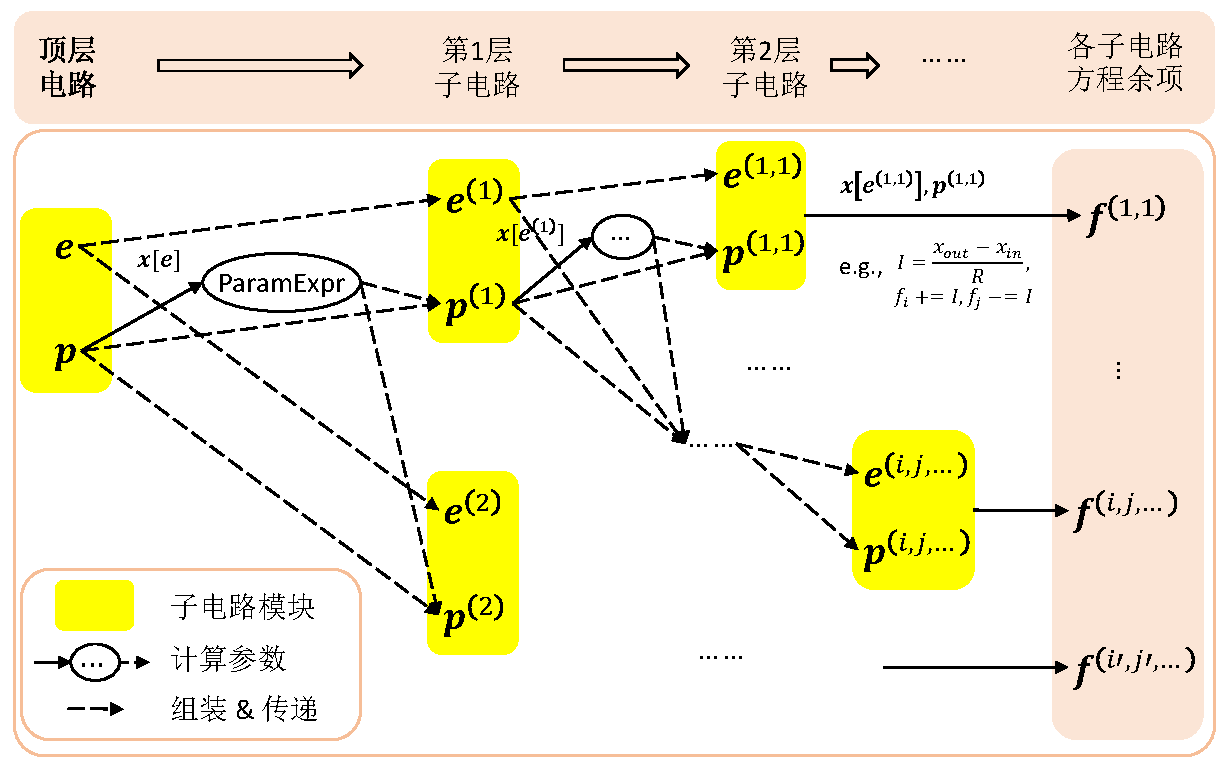
\includegraphics[width=\textwidth]{fig/static-engine.pdf}
		\caption{Existing method using static parameters}
		\label{fig:static-engine}
	\end{subfigure}
	\begin{subfigure}{0.49\textwidth}
		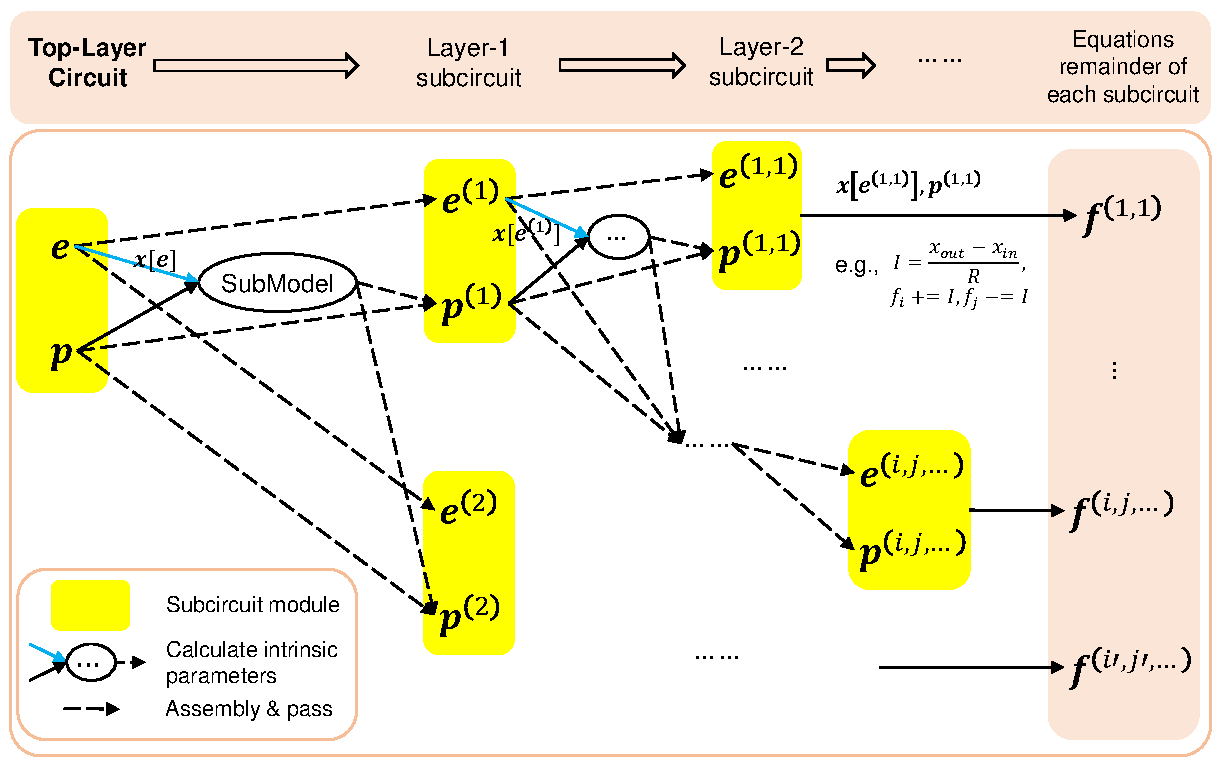
\includegraphics[width=\textwidth]{fig/computational-graph.pdf}
		\caption{Computational graph using dynamic parameters}
		\label{fig:computational-graph}
	\end{subfigure}
	\caption{Equations system constructor for hierarchical circuits: existing method v.s. computational graph. Each computing unit corresponds to a subcircuit, which can be decomposed into smaller subcircuits --- the smallest granularity subcircuit are the "basic elements". $\bm{e}^{(\cdots)}$ denotes the internal and external nodes of a subcircuit, $\bm{x}$ a generalized signal, such as node bias or branch current, $\bm{p}^{(\cdots)}$ the input parameters of a subcircuit, for example, the device size (alternatively, a non-linear capacitance, inductance, or current value of a basic element, functioning as a dynamic parameter), and $\bm{f}^{(\cdots)}$ the contribution of a subcircuit to the remainder of the simulation equations. Calculation of the Jacobian matrix is omitted in this schematic. In the existing method, a lower-layer parameter of a circuit module does not depend on the signal value ($\bm{x}[\bm{e}]$), and calculation of ParamExpr can be completed when the netlist is built. In the computational graph method, the dynamic parameters are derived from the {\color{capri}intrinsic parameters} output by SubModel --- these parameters are obtained at the calculation runtime of the systems of equations.}
	\label{fig:equations-system-constructor}
\end{figure}
For any $N$ generalized signals (i.e., equation unknowns) $\bm{x}\in\mr^N$ and $M$ signal-independent input variables or parameters $\bm{p}\in\mr^M$, the mathematical meaning of circuit simulation is constructing and solving the following conservation algebraic differential equations \cite{najm2010circuit,gunther2005modelling,hu2020adjoint}
\begin{equation}\label{eq:flat-equation}
\bm{f}(\bm{\dot{x}}(t), \bm{x}(t), \bm{p})
\triangleq\frac{\ud\bm{Q}(\bm{x},\bm{p})}{\ud t}+\bm{F}(\bm{x},\bm{p})
=\bm{0},\tag{Eq (Flat)}
\end{equation}
where, $\bm{Q}$ denotes the dynamic part of the remainder of the equation (e.g., the charge of different capacitors and magnetic flux of different inductors) and $\bm{F}$ denotes the static part of the remainder of the equation (e.g., the total input DC current at each node and the voltage drop equation). Modern simulators tend to decompose and construct \ref{eq:flat-equation} based on circuit hierarchy, which are easier to understand and parallelize:
\begin{equation}\label{eq:hierarchical-equation}
\begin{split}
\bm{f}(\bm{\dot{x}},\bm{x},\bm{p})
& = \bm{f}^{(1)}(\bm{\dot{x}}^{(1)},\bm{x}^{(1)},\bm{p}^{(1)})
+ \bm{f}^{(2)}(\bm{\dot{x}}^{(2)},\bm{x}^{(2)},\bm{p}^{(2)})
+ \cdots \\
& = \bm{f}^{(1,1)}+\bm{f}^{(1,2)}+\cdots+\bm{f}^{(2,1)}+\bm{f}^{(2,2)}+\cdots, \\
& \cdots
\end{split}\tag{Eq (Hierarchical)}
\end{equation}
where, $\bm{x}^{(i)}$, $\bm{p}^{(i)}$, and $\bm{f}^{(i)}$ respectively denote the input signals, parameters or variables, and contribution to the remainder of the equation of subcircuit $i$ of the given circuit. The overlapping part between $\bm{x}^{(i)}$ and $\bm{f}^{(i)}$ depends on the common nodes of the subcircuits. As shown in \ref{eq:hierarchical-equation}, $\bm{f}^{(i)}$ may be further decomposed into $\bm{f}^{(i,1)},\bm{f}^{(i,2)},\cdots$ as required.

Note that \ref{eq:flat-equation} represents only transient (TRAN) equations, and \ref{eq:flat-equation} is usually discretized in the time direction during numerical solution. At each time step, the system of algebraic equations is solved using the Newton-Raphson method
\cite[Section 7.1]{fijnvandraat2002time}
\[
\text{ Solve }\bm{x},\text{ Subject to }
\frac{1}{\beta\Delta t}\bm{Q}(\bm{x},\bm{p})+F(\bm{x},\bm{p})+\bm{b}=\bm{0},
\]
where $\bm{Q},\bm{F}$, and sparse Jacobian matrix $\nabla_{\bm{x}}\bm{Q},\nabla_{\bm{x}}\bm{F}$ need to be repeatedly calculated. For other types of simulation such as DC analysis and AC small signal analysis, \ref{eq:flat-equation} must be converted (Appendix \ref{appendix:TRAN-to-AC-equation}). Because the processing of each analysis equation is similar, the following uses TRAN analysis and a simple JSON netlist subcircuit definition (Code \ref{lst:size-dependent-resistor}) as an example to describe how to denote the calculation of $\bm{Q}^{(\cdots)},\bm{F}^{(\cdots)}$, $\nabla_{\bm{x}^{(\cdots)}\text{ or }\bm{p}^{(\cdots)}}\bm{Q}^{(\cdots)}$, and $\nabla_{\bm{x}^{(\cdots)}\text{ or }\bm{p}^{(\cdots)}}\bm{F}^{(\cdots)}$ in hierarchical circuit simulation as the forward and backward pass of a computational graph (Figure \ref{fig:computational-graph}).

\subsection{Subcircuit Module Definition in JSON Format Netlist}
\label{subsec:subckt-module-definition}
Similar to Verilog-AMS \cite[Section 6]{verilog2014verilog}, we define a circuit module that contains five parts of information (Table \ref{tab:subckt-module-definition}): (1) external nodes; (2) internal nodes; (3) input parameters; (4) decomposition of internal subcircuits; and (5) intrinsic parameters.
\begin{lstlisting}[language=json,basicstyle=\small,numbers=none,
caption={User-defined subcircuit named SizeDepResistor in the netlist: a resistor whose resistance is size-dependent},
label=lst:size-dependent-resistor]
"SizeDepResistor":{ # Define the subcircuit module.
  "ExternalNodes":["l","r"],
  "InputParams":["Rlength","Rwidth"],
  "InternalNodes":[],
  "SubModel":{
    "Expr":"[1e2*Rlength/Rwidth,]",
    "IntrinsicParams":["RValue"]
  },
  "Schematic":{
    # Instantiate each subcircuit or element in the module.
    "instanceR":{
      "MasterName":"resistor",
      "ExternalNodes":{"left":"l","right":"r"},
      "InputParams":{"resistance":"RValue"}
    }
  }
}
\end{lstlisting}
\begin{table}[htbp]
\centering
\caption{Subcircuit module definition}\label{tab:subckt-module-definition}
\begin{tabular}{l|l|l|l}
	\hline
	& \multicolumn{1}{c|}{Content} & \multicolumn{1}{c|}{Field} &\\
	\hline
	\multirow{4}{*}{\begin{tabular}[c]{@{}r@{}}Structural information\\{\small(dictionary+list)}\end{tabular}}
	& List of external node names & ExternalNodes & Required \\
	& List of internal node names &InternalNodes & Required \\
	& List of input parameter names &InputParams & Required \\
	& Internal subcircuit decomposition & Schematic & Required \\
	\hline
	\begin{tabular}[c]{@{}r@{}}Behavioral information\\{\small(differentiable function)}\end{tabular}
      & \begin{tabular}[c]{@{}l@{}}Submodel for calculating\\intrinsic parameters\end{tabular}& SubModel      & Optional \\
	\hline
\end{tabular}
\end{table}
The "Schematic" field represents internal subcircuit decomposition, which includes zero or more instantiation statements of subcircuits/devices. Each instantiation statement in "Schematic" is composed of (1) an instance name; (2) a class name (or master name); (3) external node connections; and (4) input parameter values. Code \ref{lst:size-dependent-resistor} provides an example, where the subcircuit decomposition part involves only one instance.
\begin{itemize}[partopsep=0pt,topsep=0pt,itemsep=0pt,parsep=0pt]
\item "instanceR" indicates the instance name.
\item "MasterName" indicates that the instance is of the "resistor" class. The class, or master, can be a subcircuit module or a type of built-in supported basic element.
\item "ExternalNodes" indicates that the two external nodes "left" and "right" of the instance are respectively connected to ports "l" and "r" of the module, i.e., "SizeDepResistor" here. In general case, the nodes connected to each instance in "Schematic" must come from "ExternalNodes" and "InternalNodes" of the given module.
\item "InputParams" indicates that the parameter of the instance is the internal variable "RValue" calculated by "SubModel". The parameters referenced by the instance in "Schematic" must come from:
(1) global variables; (2) "InputParams" of the module; (3) "IntrinsicParams" under "SubModel" (if any) of the model.
\end{itemize}
For more information about SubModel and its functionality, see Section \ref{subsec:EvalCompositeSubCkt}.

\subsection{Representation of Subcircuit Module Instances in a Program}
\label{subsec:subckt-instance-data-structure}
The subcircuit definition should be compiled into an appropriate hierarchical data structure (Figure \ref{fig:subckt-instance-data-structure}) so that the equations system constructor can efficiently invoke subcircuit modules. A compiled subcircuit module contains two parts: common computation rules of subcircuits of the same master (Table \ref{tab:BasicCompositeSubCktRule}) and instance private data (Table \ref{tab:CompositeSubCkt})
\begin{figure}[htpb]
\centering
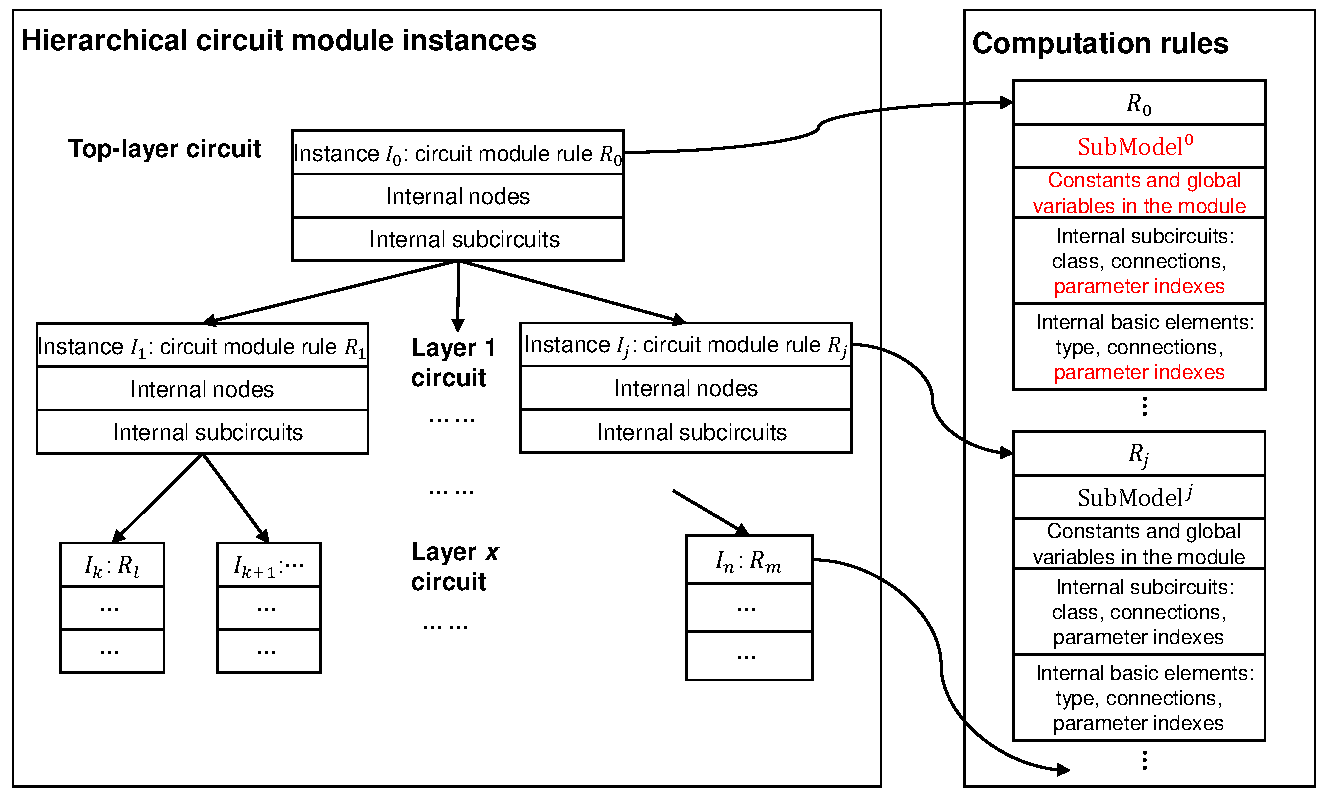
\includegraphics[width=0.8\textwidth]{fig/subckt-instance-data-structure.pdf}
\caption{Schematic diagram of hierarchical subcircuit module instances and computation rules. {\color{red}Text in red} indicates the parts that mark the differences from the existing method \cite{tcherniaev2003transistor}.
  Because the existing method does not need to support dynamic parameters, it is only necessary to store the fixed parameters of the devices in the computation rules of each circuit module. However, because the proposed method requires that parameters passed to lower-layer instances and devices be calculated during runtime, parameter indexing is necessary.}
\label{fig:subckt-instance-data-structure}
\end{figure}
\begin{table}[htbp]
\centering
\caption{Instance private data of a subcircuit module}\label{tab:CompositeSubCkt}
\begin{tabular}{l|l}
	\hline
	\multicolumn{1}{c|}{Symbol} & \multicolumn{1}{c}{Description}\\
	\hline
	rule        & Pointer to the corresponding computation rules (Table \ref{tab:BasicCompositeSubCktRule}) \\
    \textbf{in} & Internal nodes \\
	subckts     & Pointers to lower-layer subcircuit instances \\
	\hline
\end{tabular}
\end{table}
\begin{table}[htbp]
\centering
\caption{Computation rule of a subcircuit module}\label{tab:BasicCompositeSubCktRule}
\begin{tabular}{l|l}
	\hline
	\multicolumn{1}{c|}{Symbol} & \multicolumn{1}{c}{Description}\\
	\hline
	\textbf{c}       & Constants\\
	\textbf{gv}      & Global variables\\
	SubModel         & SubModel for calculating intrinsic parameters \\
	SubCktsInfo      & Lower-layer subcircuit nodes and parameter indexes \\
	BasicElementInfo & Basic element nodes and parameter indexes \\
	\hline
\end{tabular}
\end{table}
There are a few points to note:
\begin{enumerate}[partopsep=0pt,topsep=0pt,itemsep=0pt,parsep=0pt]
\item The external nodes of a subcircuit are from its upper-layer subcircuits. The top-layer circuit is a closed system without external nodes.
\item Subcircuit instances may share external nodes with one another, but the internal nodes of a subcircuit instance are exclusive to itself. When instantiating a subcircuit, ensure that its internal nodes do not conflict with each other.
\item Global variables and system signals $\bm{x}$ are globally visible to all subcircuit modules. Only the indexes \textbf{gv} of global variables need to be stored in the module's computation rules (Table \ref{tab:BasicCompositeSubCktRule}). The internal and external nodes of a module are also indexed for easy storage and passing.
\item If interactive analysis and debugging require more support information, the subcircuit master names, internal and external node parameter names, and lower-layer subcircuit instantiation statements can be added to a computation rule (Table \ref{tab:BasicCompositeSubCktRule}). Additionally, the input parameters can be dynamically recorded in an instance (Table \ref{tab:CompositeSubCkt}).
\end{enumerate}

\subsection{Instance Compilation from Subcircuit Module Definition}
\label{subsec:subckt-module-compilation}
A JSON netlist file can be parsed using JSON parser tools available in a variety of programming languages. The compilation of the subcircuit module definition (Section \ref{subsec:subckt-module-definition}) involves two steps:
\begin{enumerate}[partopsep=0pt,topsep=0pt,itemsep=0pt,parsep=0pt]
  \item Compile the computation rules of all subcircuit modules (Figure \ref{fig:compile-subckt-rule}). SubModel finishes parsing and compilation based on the compiler's implementation. To process other structural information (i.e., to create nodes and parameters indexes), only basic algorithms and data structures such as lists and dictionaries are needed.
\item Recursively instantiate the hierarchical circuit modules (Figure \ref{fig:cktrule-to-subckt}).
  The indexes of the input nodes are offset by $n=0$ if the instantiation program was launched at top layer circuit. The proposed method ensures that the internal nodes of each subcircuit module are independent of each other.
\end{enumerate}
\begin{figure}[htpb]
\centering
\begin{subfigure}{0.59\textwidth}
	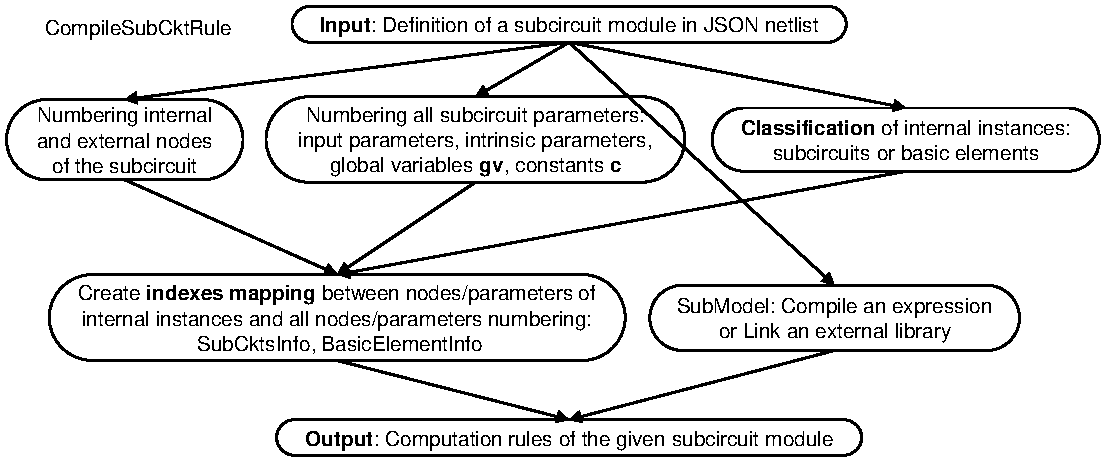
\includegraphics[width = \textwidth]{fig/compile-subckt-rule.pdf}
	\caption{Compiling the computation rules of a module}
	\label{fig:compile-subckt-rule}
\end{subfigure}
\begin{subfigure}{0.35\textwidth}
	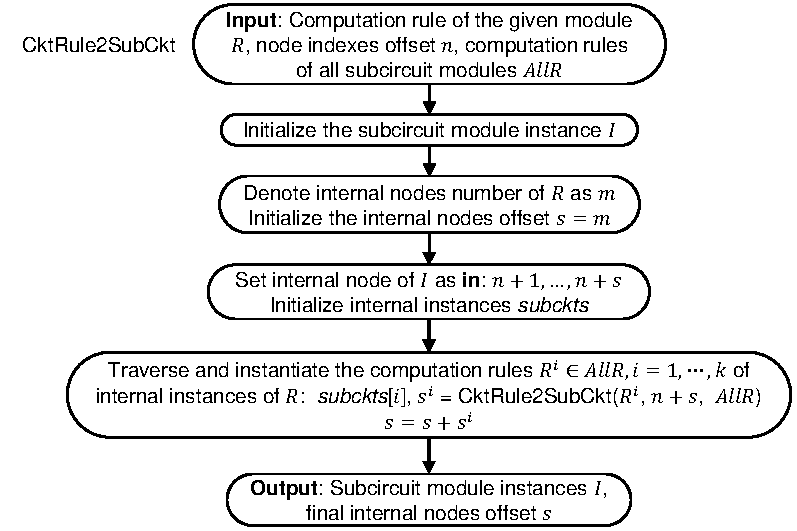
\includegraphics[width = \textwidth]{fig/cktrule-to-subckt.pdf}
	\caption{Recursive instantiation}
	\label{fig:cktrule-to-subckt}
\end{subfigure}
\caption{Compiling circuit modules}
\label{fig:subckt-module-compilation}
\end{figure}
Note that the internal subcircuit decomposition of a circuit module may include both basic elements and other circuit modules defined in the netlist. As such, the compiler should be able to distinguish between these two types of instances before it creates indexes for nodes and parameters. This is in addition to the compiler being able to check that there are no circular definitions of subcircuit class, undefined subcircuit modules, disconnected subcircuits, and unused nodes in the circuit.
\paragraph{Basic Elements}
\addcontentsline{toc}{subsubsection}{\ \ \ \ Basic Elements}
Basic elements are the smallest grained subcircuits without internal nodes or devices. Table \ref{tab:basic-elements-partial-list} provides a brief list of supported basic elements. To add a type of basic elements, we need to define the electrical response function for each analysis and then provide information such as external nodes and input parameters to the compiler.
\begin{table}[htpb]
\centering
\caption{Supported basic elements}
\label{tab:basic-elements-partial-list}
\begin{tabular}{l|l|l|l}
	\hline
	\multicolumn{1}{c}{MasterName}   & \multicolumn{1}{|c|}{ExternalNodes} &
	\multicolumn{1}{c|}{InputParams} & Remarks             \\
	\hline
	resistor   & left,right              & resistance  & Resistor           \\
	capacitor  & input,output            & capacitance & Capacitor           \\
	inductor   & input,output            & inductance  & Inductor           \\
	CS         & input,output            & current     & Current Source           \\
	VS         & input,output            & voltage     & Voltage Source           \\
	VCCS       & left,right,input,output & MF          & Voltage Controlled Current Source   \\
	CCCS       & iorigin,input,output    & MF          & Current Controlled Current Source   \\
	VCVS       & left,right,input,output & MF          & Voltage Controlled Voltage Source   \\
	CCVS       & iorigin,input,output    & MF          & Current Controlled Voltage Source   \\
	\hline
\end{tabular}
\end{table}

According to the modified nodal analysis method \cite{ho1975modified}, the basic elements of the voltage source type must take the branch current as one of the degrees of freedom --- this branch current is processed as an external GALV node in the compiler. At compile time, the GALV node needs to be added to the upper-layer module as an internal node. A generalized external GALV node can also be added for basic elements of a non-voltage source type such as resistors, to indicate the current flowing through the element branch. Consider a TRAN analysis example, with the resistance of the resistor denoted as $R$, the left and right nodes $l$ and $r$, the voltage value $x_l$ and $x_r$, and with or without the GALV node and current value $i,x_i$, we can present the remainder of the equation corresponding to the resistor using a sparse vector as follows:
\begin{description}
\item[Without external GALV:] $\bm{Q}=\bm{0},\bm{F}=[(l,-\frac{x_l-x_r}{R}),(r,\frac{x_l-x_r}{R})]$
\item[With external GALV:] $\bm{Q}=\bm{0},\bm{F}=[(l,-x_i),(r,x_i),(i,x_r-x_l+R\cdot x_i)]$
\end{description}
The two equations correspond to the so-called "element stamps" of the same type of elements described in \cite[Section 2.4.4]{najm2010circuit}. We may also consider them as two network analysis methods \cite{ho1975modified,hachtel1971sparse} for the same type of elements, which requires the support of both the compiler and the equations system constructor. For different analysis type, the calculation of remainder terms and that of the gradients in the basic element simulation equation must be distinguished --- we will not discuss that in detail here.

\subsection{Execution: Forward and Backward Pass of a Computational Graph}\label{subsec:EvalCompositeSubCkt}
Each basic computing unit of the computational graph (Figure \ref{fig:computational-graph}) corresponds to a subcircuit instance. When the subcircuit is invoked in a computational graph, the computing unit first takes external nodes and input variables as input from upper layer circuit. The compute unit then traverses the internal subcircuit and basic devices to calculate the equation remainder and the signal and variable gradients. Finally, these results are returned to the upper layer. See Algorithm \ref{alg:EvalCompositeSubCkt} for the internal process details.

Figure \ref{fig:EvalCompositeSubCkt} shows steps 1 to 5 of Algorithm \ref{alg:EvalCompositeSubCkt}, where \textbf{en}, \textbf{ip}, \textbf{in}, \textbf{gv}, and \textbf{intrp} stand for external nodes, input parameters, internal nodes, global variables, and intrinsic parameters, respectively. The internal and external nodes \textbf{en},\textbf{in} of the circuit may be used to index the generalized signal values $\bm{x}[\textbf{en}],\bm{x}[\textbf{in}]$, respectively. The variables/parameters $\bm{p}$ involved in the circuit module consists of four parts: \textbf{ip}, \textbf{gv}, \textbf{intrp}, and \textbf{c}.

\begin{algorithm}[h]
\caption{Calling a Subcircuit\\
    equations remainder, signal gradient, variable gradient = \\
    {\color{white}\tiny PLACEHOLDER}EvalCompositeSubCkt($\bm{x}$,ckt,\textbf{en},\textbf{ip})
    }
\label{alg:EvalCompositeSubCkt}
\SetAlgoLined
Input: System signals $\bm{x}$, subcircuit instance ckt,
  external node indexes \textbf{en}, input parameters \textbf{ip}\;
\# Internal information of ckt: Internal nodes \textbf{in}, SubModel, global variables \textbf{gv}, constants \textbf{c}\;
1. Assemble the internal nodes \textbf{in} and external nodes \textbf{en} of ckt, resulting in \textbf{nodes}=[\textbf{en},\textbf{in}]\;
2. Calculate the intrinsic parameters according to the internal and external signals and input parameters: \textbf{intrp} = SubModel($\bm{x}$[\textbf{nodes}],\textbf{ip})\;
3. Assemble all variables and parameters of ckt, resulting in \textbf{params}= [\textbf{ip},\textbf{intrp},\textbf{gv},\textbf{c}]\;
4. Extract the external nodes \textbf{suben}$\subset$\textbf{nodes} and input parameters \textbf{subip}$\subset$\textbf{params} of each subcircuit (subckt) in ckt from \textbf{nodes},\textbf{params}, and call EvalCompositeSubCkt($\bm{x}$,subckt,\textbf{suben},\textbf{subip})\;
5. Extract the external nodes and input parameters of each basic element in ckt from \textbf{nodes},\textbf{params}, and calculate the equation remainder and gradient of each basic element\;
6. Collect the remainder terms of all equations in steps 4 and 5\;
7. Propagate signal and variable gradients of lower-layer subcircuits and basic elements backward according to the index mapping of steps 1 to 5\;
Output: Equation remainder, signal gradient, variable gradient
\end{algorithm}
\begin{figure}[htpb]
\centering
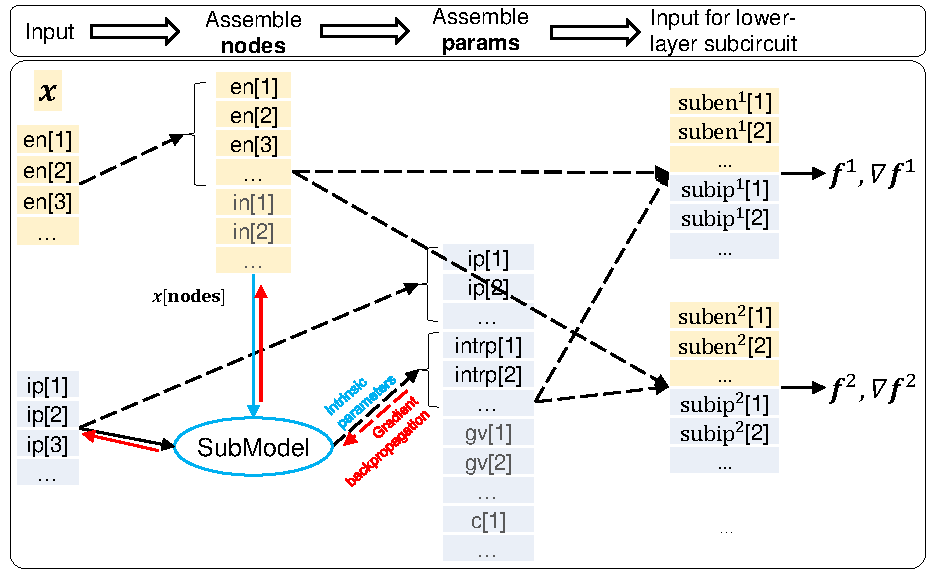
\includegraphics[width=0.7\textwidth]{fig/EvalCompositeSubCkt.pdf}
\caption{Schematic diagram of steps 1 to 5 of Algorithm \ref{alg:EvalCompositeSubCkt}, also a zoom-in view of the calls to the top-layer to layer-1 subcircuits in Figure \ref{fig:computational-graph}. In the existing method, the input and intrinsic parameters are computed at compile time, and no gradient of parameters are propagated backward at runtime.}
\label{fig:EvalCompositeSubCkt}
\end{figure}

\paragraph{SubModel and Intrinsic Parameters}
\addcontentsline{toc}{subsubsection}{\ \ \ \ SubModel and Internal Parameters}
In the computational graph, SubModel takes the internal and external signals and input parameters of the module as inputs, and outputs all \textit{intrinsic parameters} via \textbf{intrp}=SubModel(\textbf{signals},\textbf{ip}), where \textbf{nodes}=[\textbf{en},\textbf{in}], \textbf{signals}=$\bm{x}[\textbf{nodes}]$,
which can be passed to the lower-layer subcircuits and basic elements.
This setup is based on the Assumption \ref{assumption:intrinsic-params-dependencies}: "The behavior of a circuit module is and only is determined by the internal and external signals as well as input variables." Thus, for a SubModel, there is no need to perceive the internal signals of lower-layer subcircuits nor the node signals or parameters of other irrelevant modules. This setting can cover a considerably wide range of nonlinear effects and is easy to program.
\begin{assumption}\label{assumption:intrinsic-params-dependencies}
The intrinsic parameters in a subcircuit module are uniquely determined by the bias signals of the internal and external nodes and the input parameters of the module.
\end{assumption}
The submodel in the circuit definition should provide sufficient information so that the compiler can register the SubModel with the common rules (Table \ref{tab:BasicCompositeSubCktRule}).
In addition, there should be some protocol between the computational graph and the SubModel for obtaining the Jacobian matrix of \textbf{intrp} with respect to \textbf{signals},\textbf{ip}
\begin{equation}\label{eq:submodel-jacobian}
J_{\textbf{s}} = \nabla_{\textbf{signals}}\textbf{intrp},
J_{\textbf{ip}}=\nabla_{\textbf{ip}}\textbf{intrp},
\end{equation}
The specific implementation depends on the programming language used. As such, details are not provided here.

\paragraph{Layer-wise Gradient Backpropagation}
\addcontentsline{toc}{subsubsection}{\ \ \ \ Layer-wise Gradient Backpropagation}
A computational graph completes the computation process by calling subcircuits. The computing logic differs from that involved in the existing method (Figure \ref{fig:equations-system-constructor}) in one major aspect: In the computational graph, the input parameters \textbf{subip} of lower-layer modules or elements come from a subset of the assembled parameters \textbf{params} (Figure \ref{fig:EvalCompositeSubCkt}). Consequently, gradient backpropagation for \textbf{subip} is required. The following describes the gradient backpropagation process in Algorithm \ref{alg:EvalCompositeSubCkt} for TRAN simulation as an example.

For TRAN analysis, the returned value of Algorithm \ref{alg:EvalCompositeSubCkt} contains the following eight items:
$\bm{Q}, \bm{F}, \nabla_{\bm{x}}\bm{Q}, \nabla_{\bm{x}}\bm{F}$,
$\nabla_{\textbf{gv}}\bm{Q}, \nabla_{\textbf{ip}}\bm{Q}$,
$\nabla_{\textbf{gv}}\bm{F}$, and $\nabla_{\textbf{ip}}\bm{F}$.
Because the gradient backpropagation of $\bm{Q}$ is the same as that of $\bm{F}$, only $\bm{Q}$ is considered for simplicity.
The computation results of all subcircuits of Algorithm \ref{alg:EvalCompositeSubCkt} are recorded as $\{\bm{Q}^{i}\}$, $\{\nabla_{\bm{x}}\bm{Q}^{i}\}$, $\{\nabla_{\textbf{gv}}\bm{Q}^{i}\}$, and $\{\nabla_{\textbf{subip}^i}\bm{Q}^{i}\}$, where the superscript $i$ denotes the sequence number of the internal subcircuit or basic element. $\bm{Q}^{i}$, $\nabla_{\bm{x}}\bm{Q}^{i}$, and $\nabla_{\textbf{gv}}\bm{Q}^{i}$ can be directly assembled as
\[
\bm{Q} = \sum_i \bm{Q}^{i},
\nabla_{\bm{x}}\bm{Q} = \sum_i \nabla_{\bm{x}}\bm{Q}^{i},
\nabla_{\textbf{gv}}\bm{Q} = \sum_i \nabla_{\textbf{gv}}\bm{Q}^{i},
\]
while the gradient backpropagation of $\nabla_{\textbf{subip}^i}\bm{Q}^{i}$ needs to be processed differently based on the index of $\textbf{subip}^i$ to \textbf{params}=[\textbf{ip},\textbf{intrp},\textbf{gv},\textbf{c}].

\begin{enumerate}[partopsep=0pt,itemsep=0pt,parsep=0pt]
\item If $\text{subip}^i[j]\in\textbf{c}$, backpropagation is not performed.
\item If $\text{subip}^i[j]\in\textbf{ip}\cup\textbf{gv}$, then $\nabla_{\text{subip}^i[j]}\bm{Q}^i$ is propagated to the corresponding $\nabla_\textbf{ip}\bm{Q}$ or $\nabla_\textbf{gv}\bm{Q}$.
\item If $\text{subip}^i[j]=\textbf{intrp}[l]$ for any index $l$ (Figure \ref{fig:EvalCompositeSubCkt}), given Assumption \ref{assumption:intrinsic-params-dependencies} and the Jacobian matrix of the intrinsic parameters with respect to the signal and input parameters (Equation \ref{eq:submodel-jacobian}), then (let $\bm{g}\triangleq\nabla_{\textbf{subip}^i[j]}\bm{Q}^{i}$)
\begin{equation}\label{eq:intrinsic-params-backward}
\nabla_{x[\textbf{nodes}]}\bm{Q}\mathrel{+}=J_{\textbf{s}}[:,l]\otimes\bm{g},
\nabla_{\textbf{ip}}\bm{Q}\mathrel{+}=J_{\textbf{ip}}[:,l]\otimes\bm{g}.
\end{equation}
where, $\otimes$ represents the outer product of two vectors.
\end{enumerate}

